\documentclass[xcolor=dvipsnames]{beamer}
\usepackage[T1]{fontenc}
\usepackage[utf8]{inputenc}
\usepackage[english,slovak]{babel}

\usepackage{amsmath}
\usepackage{amsthm}
\usetheme{Pittsburgh}
\useoutertheme{shadow}

\usepackage{graphicx}
\usepackage{caption}
\usepackage{subcaption}

\usepackage[]{algorithm2e}
\usepackage{listings}
 \setbeamercovered{transparent}
 \usepackage{cuted}
\usepackage[export]{adjustbox}
\usepackage{mathtools}

\usepackage{lipsum}

\newcommand\Wider[2][3em]{%
\makebox[\linewidth][c]{%
  \begin{minipage}{\dimexpr\textwidth+#1\relax}
  \raggedright#2
  \end{minipage}%
  }%
}

%-------------------------------------------------------------------------------------
\title{\bf Kde v umelej inteligencii a robotike treba matematiku}
\author{Michal CHOVANEC}


%\setbeamertemplate{footline}[frame number]{}
\setbeamertemplate{navigation symbols}{}


\date[EURP]{\it Október 2017}
\begin{document}

\begin{frame}
\titlepage
\centering{Fakulta riadenia a informatiky}
\end{frame}



\begin{frame}{\bf Obsah}

    \begin{itemize}
      \item Grafické karty nie sú len na hry
      \item Derivácie v riadení robota
      \item Geometrické postupnosti a samo sa učiace roboty
    \end{itemize}


\end{frame}


\begin{frame}{\bf Grafické karty nie sú len na hry}

\centering
\begin{figure}[htbp]
  \centering
    \includegraphics[scale=0.5]{../pictures/newton.jpg}
\end{figure}

\begin{figure}[htbp]
  \centering
    \includegraphics[scale=1.0]{../pictures/1080ti.jpg}
\end{figure}

\end{frame}


\begin{frame}{\bf Problém N-telies}

Spočítať dráhy veľkého (tisíce) množstva telies, ktoré na seba gravitačna pôsobia

\begin{figure}[htbp]
  \centering
    \includegraphics[scale=0.15]{n_body_problem.png}
\end{figure}

Stredoškolská podoba gravitačného zákona (pre dve telesá)
\begin{align*}
F = G\frac {m_1m_2}{r^2}
\end{align*}

Druhý newtonov zákon
\begin{align*}
F = ma
\end{align*}

\end{frame}



\begin{frame}{\bf Problém N-telies}

\begin{align*}
F &= G\frac {m_1m_2}{r^2} \\
F_{12} &= G\frac {m_1m_2}{r_{12}^3}\hat{r_{12}} \text{ vektorový tvar pre 2 telesá}\\
F_{ij} &= G\frac {m_im_j}{r_{ij}^3}\hat{r_{ij}} \text{ vektorový tvar pre telesá i,j}\\
F_{j} &= G \sum_{j \neq i} \frac {m_im_j}{r_{ij}^3}\hat{r_{ij}} \text{ výsledná sila pôsobiaca na j-te teleso}\\
\end{align*}

\end{frame}


\begin{frame}{\bf Problém N-telies}

\begin{align*}
F &= ma \\
a(t) &= \frac{F(t)}{m} \\
\frac{d^2x(t)}{dt} &= \frac{F(t)}{m}
\end{align*}
... čo sa dá previesť do ľahko naprogramovateľnej podoby

\begin{align*}
v(n) &= v(n-1) + \frac{F(n)}{m}dt \text{ rýchlosť častice}\\
x(n) &= x(n-1) + v(n)dt \text{ poloha častice}
\end{align*}

\end{frame}

\begin{frame}{\bf Problém N-telies, ukážka}

\begin{figure}[htbp]
  \centering
    \includegraphics[scale=0.2]{n_body_animation.png}
\end{figure}

\end{frame}


\begin{frame}{\bf Skalárny súčin - spracovanie obrazu}


\[
\begin{bmatrix}
    7  & 3 & 2 \\
    8  & 2 & 4 \\
    6  & 9 & 1 \\
\end{bmatrix}
\cdot
\begin{bmatrix}
    -0.125  & -0.125 & -0.125 \\
    -0.125  & 1 & -0.125 \\
    -0.125  & -0.125 & -0.125 \\
\end{bmatrix}
= \]

\begin{align*}
7\cdot(-0.125) &+ 3\cdot(-0.125) + 2\cdot(-0.125) + \\
8\cdot(-0.125) &+ 2\cdot1 + 4\cdot(-0.125) + \\
6\cdot(-0.125) &+ 9\cdot(-0.125) + 1\cdot(-0.125) = \\
&-3
\end{align*}

\end{frame}


\begin{frame}{\bf Skalárny súčin - spracovanie obrazu}
\Wider[4em]
{

\begin{minipage}[r]{0.5\textwidth}

    \begin{figure}[htbp]
      \centering
        \includegraphics[scale=0.18]{fil_original.jpg}
    \end{figure}

    \begin{figure}[htbp]
      \centering
        \includegraphics[scale=0.18]{fil_av.jpg}
    \end{figure}

\end{minipage}%
\hfill
\begin{minipage}[c]{0.5\textwidth}

\[
\begin{bmatrix}
    1  & 1 & 1 \\
    1  & 1 & 1 \\
    1  & 1 & 1 \\
\end{bmatrix}
\]

\end{minipage}%

}
\end{frame}






\begin{frame}{\bf Skalárny súčin - spracovanie obrazu}
\Wider[4em]
{

\begin{minipage}[r]{0.5\textwidth}

    \begin{figure}[htbp]
      \centering
        \includegraphics[scale=0.18]{fil_original.jpg}
    \end{figure}

    \begin{figure}[htbp]
      \centering
        \includegraphics[scale=0.18]{fil_sharp.jpg}
    \end{figure}

\end{minipage}%
\hfill
\begin{minipage}[c]{0.5\textwidth}

\[
\begin{bmatrix}
    0  & -1 & 0 \\
    -1  & 5 & -1 \\
    0  & -1 & 0 \\
\end{bmatrix}
\]

\end{minipage}%

}
\end{frame}




\begin{frame}{\bf Skalárny súčin - spracovanie obrazu}
\Wider[4em]
{

\begin{minipage}[r]{0.5\textwidth}

    \begin{figure}[htbp]
      \centering
        \includegraphics[scale=0.18]{fil_original.jpg}
    \end{figure}

    \begin{figure}[htbp]
      \centering
        \includegraphics[scale=0.18]{fil_edges.jpg}
    \end{figure}

\end{minipage}%
\hfill
\begin{minipage}[c]{0.5\textwidth}

\[
\begin{bmatrix}
    -0.125  & -0.125 & -0.125 \\
    -0.125  & 1 & -0.125 \\
    -0.125  & -0.125 & -0.125 \\
\end{bmatrix}
\]

\end{minipage}%

}
\end{frame}





\begin{frame}{\bf Skalárny súčin - spracovanie obrazu}
\Wider[4em]
{

\begin{minipage}[r]{0.5\textwidth}

    \begin{figure}[htbp]
      \centering
        \includegraphics[scale=0.18]{fil_original.jpg}
    \end{figure}

    \begin{figure}[htbp]
      \centering
        \includegraphics[scale=0.18]{fil_edges_h.jpg}
    \end{figure}

\end{minipage}%
\hfill
\begin{minipage}[c]{0.5\textwidth}

\[
\begin{bmatrix}
    -1  & -2 & -1 \\
    0  & 0 & 0 \\
    1  & 2 & 1 \\
\end{bmatrix}
\]

\end{minipage}%

}
\end{frame}

\begin{frame}{\bf Derivácie v riadení robota}

\begin {itemize}
\item PID regulátory - 90\% riadenia výrobných liniek
\item stabilizácia robota pomocou gyroskopu a PD regulátora
\end {itemize}

\begin{figure}[htbp]
  \centering
    \includegraphics[scale=0.4]{controller.eps}
\end{figure}

\end{frame}


\begin{frame}{\bf Derivácie v riadení robota}
\begin{align*}
\text{ak platí } {\bf F = ma} \text{ nie } F = mv
\end{align*}

\begin{align*}
u &= P\text{ chyba} + D \frac{d \text{chyba}}{dt} \\
u(n) &= Pe(n) + D(e(n) - e(n-1))
\end{align*}

\begin{figure}[htbp]
  \centering
    \includegraphics[scale=0.4]{controller.eps}
\end{figure}

\end{frame}


\begin{frame}{\bf Geometrické postupnosti a samo sa učiace roboty}

\begin{minipage}[r]{0.5\textwidth}

    \begin{figure}[htbp]
      \centering
        \includegraphics[scale=0.3]{chess.png}
    \end{figure}
    \begin{figure}[htbp]
      \centering
        \includegraphics[scale=0.1]{pacman.jpg}
    \end{figure}
\end{minipage}%
\hfill
\begin{minipage}[c]{0.5\textwidth}

\begin{itemize}
 \item Voľba najlepšiej stratégie
 \item Učenie sa z odmien a trestov
 \item Čo je to inteligencia?
\end{itemize}

\end{minipage}%


\end{frame}




\begin{frame}{\bf Geometrické postupnosti a samo sa učiace roboty}

\begin{minipage}[r]{0.5\textwidth}
    \begin{figure}[htbp]
      \centering
        \includegraphics[scale=0.3]{chess.png}
    \end{figure}
\end{minipage}%
\hfill
\begin{minipage}[c]{0.5\textwidth}
  \begin{itemize}
   \item Voľba najlepšiej stratégie
   \item Učenie sa z odmien a trestov
   \item Čo je to inteligencia?
  \end{itemize}
\end{minipage}%

... prekvapivo jednoduchá rovnica \footnotemark
\begin{align*}
Q(\text{teraz}) &= Odmena(\text{teraz}) + \gamma Q(\text{budúcnosť}) \\
Q'(s, a) &= (1-\alpha)Q(s, a) + \alpha(R(s, a) + \gamma Q(s', a'))
\end{align*}

$\gamma$ zodpovedá ze plánovanie do budúcnosti - určuje budúce dôsledky
aktuálneho rozhodnutia
\footnotetext[1]{\tiny{Online Q-Learning using Connectionist Systems, by Rummery \& Niranjan (1994)}}
\end{frame}

\begin{frame}{\bf Geometrické postupnosti a samo sa učiace roboty}

\centering
\begin{figure}[C]
   \includegraphics[scale=0.27]{../pictures/sdm_demo_desc.png}
\end{figure}

\end{frame}

%-------------------------------------------------------------------------------------
\begin{frame}{\bf Q\&A}

\begin{figure}[ht]
\begin{center}
\begin{minipage}{0.8\linewidth}
\begin{center}
 \includegraphics[width=1.0\textwidth]{../pictures/me.jpg}
\end{center}
\end{minipage}
\end{center}
\end{figure}

\url{https://github.com/michalnand/robotics}
\url{https://github.com/michalnand/machine\_learning\_new}

\centerline{michal.nand@gmail.com}

\end{frame}

\end{document}
